%        File: arfc-beamer.tex
%     Created: Sun May 5 10:00 PM 2013 C
%


%\documentclass[11pt,handout]{beamer}
\documentclass[9pt]{beamer}
\usetheme[white]{Illinois}
%\title[short title]{long title}
\title[Fuel processing simulation tool for liquid-fueled reactors]{Fuel processing simulation tool for liquid-fueled nuclear reactors \\ Preliminary Exam}
%\subtitle[short subtitle]{long subtitle}
%\subtitle[Short SubTitle]{Mostly Kittens}
%\author[short name]{long name}
\author[Andrei Rykhlevskii]{Andrei Rykhlevskii}
%\date[short date]{long date}
\date[05.05.2019]{September 5, 2019}
%\institution[short name]{long name}
\institute[UIUC]{University of Illinois at Urbana-Champaign}


\usepackage{lmodern}

%\usepackage{bbding}
\usepackage{tikz}
\usepackage{amsfonts}
\usepackage{amsmath}
\usepackage{caption}  % allows center figures caption
\usepackage{xspace}
\usepackage{notoccite}
\usepackage{graphicx}
\usepackage{animate}
\usepackage{subfigure}
\usepackage{booktabs} % nice rules for tables
\usepackage{microtype} % if using PDF
\usepackage{bigints}
\usepackage[absolute,overlay]{textpos}
%\usepackage{minted}
\usepackage{xcolor}
\usepackage{soul}
\newcommand{\hlc}[2][yellow]{{%
    \colorlet{foo}{#1}%
    \sethlcolor{foo}\hl{#2}}%
}
\newcommand{\units}[1] {\:\text{#1}}%
\newcommand{\SN}{S$_N$}%{S$_\text{N}$}%{$S_N$}%
\DeclareMathOperator{\erf}{erf}
%I need some complimentary error funcitons... 
\DeclareMathOperator{\erfc}{erfc}
%page numbers
\setbeamertemplate{page number in head/foot}[appendixframenumber]
\setbeamertemplate{caption}[numbered]
%Those icons in the references are terrible looking
\setbeamertemplate{bibliography item}[text]
\setbeamercovered{dynamic}
%%%% Acronym support

\usepackage[acronym,toc]{glossaries}
%\newacronym{<++>}{<++>}{<++>}
\newacronym[longplural={metric tons of heavy metal}]{MTHM}{MTHM}{metric ton of heavy metal}
\newacronym{ABM}{ABM}{agent-based modeling}
\newacronym{ACDIS}{ACDIS}{Program in Arms Control \& Domestic and International Security}
\newacronym{AHTR}{AHTR}{Advanced High Temperature Reactor}
\newacronym{ANDRA}{ANDRA}{Agence Nationale pour la gestion des D\'echets RAdioactifs, the French National Agency for Radioactive Waste Management}
\newacronym{ANL}{ANL}{Argonne National Laboratory}
\newacronym{ANS}{ANS}{American Nuclear Society}
\newacronym{AOA}{AOA}{Axial Offset Anomaly}
\newacronym{API}{API}{application programming interface}
\newacronym{ARE}{ARE}{Aircraft Reactor Experiment}
\newacronym{ARFC}{ARFC}{Advanced Reactors and Fuel Cycles}
\newacronym{ASME}{ASME}{American Society of Mechanical Engineers}
\newacronym{ATWS}{ATWS}{Anticipated Transient Without Scram}
\newacronym{BOL}{BOL}{Beginning of Life}
\newacronym{BDBE}{BDBE}{Beyond Design Basis Event}
\newacronym{BIDS}{BIDS}{Berkeley Institute for Data Science}
\newacronym{BWR}{BWR}{Boiling Water Reactor}
\newacronym{CAFCA}{CAFCA}{ Code for Advanced Fuel Cycles Assessment }
\newacronym{CDTN}{CDTN}{Centro de Desenvolvimento da Tecnologia Nuclear}
\newacronym{CFD}{CFD}{Computational Fluid Dynamics}
\newacronym{CEA}{CEA}{Commissariat \`a l'\'Energie Atomique et aux \'Energies Alternatives}
\newacronym{CI}{CI}{continuous integration}
\newacronym{CNEN}{CNEN}{Comiss\~{a}o Nacional de Energia Nuclear}
\newacronym{CNERG}{CNERG}{Computational Nuclear Engineering Research Group}
\newacronym{COSI}{COSI}{Commelini-Sicard}
\newacronym{COTS}{COTS}{commercial, off-the-shelf}
\newacronym{CSNF}{CSNF}{commercial spent nuclear fuel}
\newacronym{CTAH}{CTAHs}{Coiled Tube Air Heaters}
\newacronym{CUBIT}{CUBIT}{CUBIT Geometry and Mesh Generation Toolkit}
\newacronym{CURIE}{CURIE}{Centralized Used Fuel Resource for Information Exchange}
\newacronym{CR}{CR}{conversion ratio}
\newacronym{DAG}{DAG}{directed acyclic graph}
\newacronym{DANESS}{DANESS}{Dynamic Analysis of Nuclear Energy System Strategies}
\newacronym{DBE}{DBE}{Design Basis Event}
\newacronym{DESAE}{DESAE}{Dynamic Analysis of Nuclear Energy Systems Strategies}
\newacronym{DHS}{DHS}{Department of Homeland Security}
\newacronym{DOE}{DOE}{Department of Energy}
\newacronym{DRACS}{DRACS}{Direct Reactor Auxiliary Cooling System}
\newacronym{DRE}{DRE}{dynamic resource exchange}
\newacronym{DSNF}{DSNF}{DOE spent nuclear fuel}
\newacronym{DYMOND}{DYMOND}{Dynamic Model of Nuclear Development }
\newacronym{EBS}{EBS}{Engineered Barrier System}
\newacronym{EDF}{EDF}{Électricité de France}
\newacronym{EDZ}{EDZ}{Excavation Disturbed Zone}
\newacronym{EOL}{EOL}{End of Life}
\newacronym{EIA}{EIA}{U.S. Energy Information Administration}
\newacronym{EPA}{EPA}{Environmental Protection Agency}
\newacronym{EPR}{EPR}{European Pressurized Reactors}
\newacronym{EP}{EP}{Engineering Physics}
\newacronym{EU}{EU}{European Union}
\newacronym{FCO}{FCO}{Fuel Cycle Options}
\newacronym{FCT}{FCT}{Fuel Cycle Technology}
\newacronym{FEHM}{FEHM}{Finite Element Heat and Mass Transfer}
\newacronym{FEPs}{FEPs}{Features, Events, and Processes}
\newacronym{FHR}{FHR}{Fluoride-Salt-Cooled High-Temperature Reactor}
\newacronym{FLiBe}{FLiBe}{Fluoride-Lithium-Beryllium}
\newacronym{FP}{FP}{Fission Product}
\newacronym{FTC}{FTC}{fuel temperature coefficient}
\newacronym{GDSE}{GDSE}{Generic Disposal System Environment}
\newacronym{GDSM}{GDSM}{Generic Disposal System Model}
\newacronym{GENIUSv1}{GENIUSv1}{Global Evaluation of Nuclear Infrastructure Utilization Scenarios, Version 1}
\newacronym{GENIUSv2}{GENIUSv2}{Global Evaluation of Nuclear Infrastructure Utilization Scenarios, Version 2}
\newacronym{GENIUS}{GENIUS}{Global Evaluation of Nuclear Infrastructure Utilization Scenarios}
\newacronym{GPAM}{GPAM}{Generic Performance Assessment Model}
\newacronym{GRSAC}{GRSAC}{Graphite Reactor Severe Accident Code}
\newacronym{GUI}{GUI}{graphical user interface}
\newacronym{HFP}{HFP}{hot full power}
\newacronym{HLW}{HLW}{high level waste}
\newacronym{HPC}{HPC}{high-performance computing}
\newacronym{HTC}{HTC}{high-throughput computing}
\newacronym{HTGR}{HTGR}{High Temperature Gas-Cooled Reactor}
\newacronym{HZP}{HZP}{hot zero power}
\newacronym{IAEA}{IAEA}{International Atomic Energy Agency}
\newacronym{IEMA}{IEMA}{Illinois Emergency Mangament Agency}
\newacronym{IHLRWM}{IHLRWM}{International High Level Radioactive Waste Management}
\newacronym{INL}{INL}{Idaho National Laboratory}
\newacronym{IPRR1}{IRP-R1}{Instituto de Pesquisas Radioativas Reator 1}
\newacronym{IRP}{IRP}{Integrated Research Project}
\newacronym{ISFSI}{ISFSI}{Independent Spent Fuel Storage Installation}
\newacronym{ISRG}{ISRG}{Independent Student Research Group}
\newacronym{JFNK}{JFNK}{Jacobian-Free Newton Krylov}
\newacronym{LANL}{LANL}{Los Alamos National Laboratory}
\newacronym{LBNL}{LBNL}{Lawrence Berkeley National Laboratory}
\newacronym{LCOE}{LCOE}{levelized cost of electricity}
\newacronym{LEU}{LEU}{low-enriched uranium}
\newacronym{LDRD}{LDRD}{laboratory directed research and development}
\newacronym{LFR}{LFR}{Lead-Cooled Fast Reactor}
\newacronym{LLNL}{LLNL}{Lawrence Livermore National Laboratory}
\newacronym{LMFBR}{LMFBR}{Liquid Metal Fast Breeder Reactor}
\newacronym{LOFC}{LOFC}{Loss of Forced Cooling}
\newacronym{LOHS}{LOHS}{Loss of Heat Sink}
\newacronym{LOLA}{LOLA}{Loss of Large Area}
\newacronym{LP}{LP}{linear program}
\newacronym{LWR}{LWR}{Light Water Reactor}
\newacronym{MAGNOX}{MAGNOX}{Magnesium Alloy Graphie Moderated Gas Cooled Uranium Oxide Reactor}
\newacronym{MA}{MA}{minor actinide}
\newacronym{MCNP}{MCNP}{Monte Carlo N-Particle code}
\newacronym{MCFR}{MCSFR}{Molten Chloride Fast Reactor}
\newacronym{MILP}{MILP}{mixed-integer linear program}
\newacronym{MIT}{MIT}{the Massachusetts Institute of Technology}
\newacronym{MOAB}{MOAB}{Mesh-Oriented datABase}
\newacronym{MOOSE}{MOOSE}{Multiphysics Object-Oriented Simulation Environment}
\newacronym{MOSART}{MOSART}{Molten Salt Actinide Recycler and Transmuter}
\newacronym{MOX}{MOX}{mixed oxide}
\newacronym{MPI}{MPI}{Message Passing Interface}
\newacronym{MSBR}{MSBR}{Molten Salt Breeder Reactor}
\newacronym{MSFR}{MSFR}{Molten Salt Fast Reactor}
\newacronym{MSRE}{MSRE}{Molten Salt Reactor Experiment}
\newacronym{MSR}{MSR}{Molten Salt Reactor}
\newacronym{MTC}{MTC}{moderator temperature coefficient}
\newacronym{NAGRA}{NAGRA}{National Cooperative for the Disposal of Radioactive Waste}
\newacronym{NEAMS}{NEAMS}{Nuclear Engineering Advanced Modeling and Simulation}
\newacronym{NEUP}{NEUP}{Nuclear Energy University Programs}
\newacronym{NFCSim}{NFCSim}{Nuclear Fuel Cycle Simulator}
\newacronym{NGNP}{NGNP}{Next Generation Nuclear Plant}
\newacronym{NMWPC}{NMWPC}{Nuclear MW Per Capita}
\newacronym{NNSA}{NNSA}{National Nuclear Security Administration}
\newacronym{NPP}{NPP}{Nuclear Power Plant}
\newacronym{NPRE}{NPRE}{Department of Nuclear, Plasma, and Radiological Engineering}
\newacronym{NQA1}{NQA-1}{Nuclear Quality Assurance - 1}
\newacronym{NRC}{NRC}{Nuclear Regulatory Commission}
\newacronym{NSF}{NSF}{National Science Foundation}
\newacronym{NSSC}{NSSC}{Nuclear Science and Security Consortium}
\newacronym{NUWASTE}{NUWASTE}{Nuclear Waste Assessment System for Technical Evaluation}
\newacronym{NWF}{NWF}{Nuclear Waste Fund}
\newacronym{NWTRB}{NWTRB}{Nuclear Waste Technical Review Board}
\newacronym{OCRWM}{OCRWM}{Office of Civilian Radioactive Waste Management}
\newacronym{OOP}{OOP}{Object-Oriented Programming}
\newacronym{ORION}{ORION}{ORION}
\newacronym{ORNL}{ORNL}{Oak Ridge National Laboratory}
\newacronym{PARCS}{PARCS}{Purdue Advanced Reactor Core Simulator}
\newacronym{PBAHTR}{PB-AHTR}{Pebble Bed Advanced High Temperature Reactor}
\newacronym{PBFHR}{PB-FHR}{Pebble-Bed Fluoride-Salt-Cooled High-Temperature Reactor}
\newacronym{PEI}{PEI}{Peak Environmental Impact}
\newacronym{PH}{PRONGHORN}{PRONGHORN}
\newacronym{PRIS}{PRIS}{Power Reactor Information System}
\newacronym{PRKE}{PRKE}{Point Reactor Kinetics Equations}
\newacronym{PSPG}{PSPG}{Pressure-Stabilizing/Petrov-Galerkin}
\newacronym{PWAR}{PWAR}{Pratt and Whitney Aircraft Reactor}
\newacronym{PWR}{PWR}{Pressurized Water Reactor}
\newacronym{PyNE}{PyNE}{Python toolkit for Nuclear Engineering}
\newacronym{PyRK}{PyRK}{Python for Reactor Kinetics}
\newacronym{QA}{QA}{quality assurance}
\newacronym{RDD}{RD\&D}{Research Development and Demonstration}
\newacronym{RD}{R\&D}{Research and Development}
\newacronym{REE}{REE}{rare earth element}
\newacronym{RELAP}{RELAP}{Reactor Excursion and Leak Analysis Program}
\newacronym{RIA}{RIA}{Reactivity Insertion Accident}
\newacronym{RIF}{RIF}{Region-Institution-Facility}
\newacronym{SFR}{SFR}{Sodium-Cooled Fast Reactor}
\newacronym{SINDAG}{SINDA{\textbackslash}G}{Systems Improved Numerical Differencing Analyzer $\backslash$ Gaski}
\newacronym{SKB}{SKB}{Svensk K\"{a}rnbr\"{a}nslehantering AB}
\newacronym{SNF}{SNF}{spent nuclear fuel}
\newacronym{SNL}{SNL}{Sandia National Laboratory}
\newacronym{STC}{STC}{specific temperature change}
\newacronym{SUPG}{SUPG}{Streamline-Upwind/Petrov-Galerkin}
\newacronym{SWF}{SWF}{Separations and Waste Forms}
\newacronym{SWU}{SWU}{Separative Work Unit}
\newacronym{TAP}{TAP}{Transatomic Power}
\newacronym{TRIGA}{TRIGA}{Training Research Isotope General Atomic}
\newacronym{TRISO}{TRISO}{Tristructural Isotropic}
\newacronym{TSM}{TSM}{Total System Model}
\newacronym{TSPA}{TSPA}{Total System Performance Assessment for the Yucca Mountain License Application}
\newacronym{ThOX}{ThOX}{thorium oxide}
\newacronym{UFD}{UFD}{Used Fuel Disposition}
\newacronym{UML}{UML}{Unified Modeling Language}
\newacronym{UOX}{UOX}{uranium oxide}
\newacronym{UQ}{UQ}{uncertainty quantification}
\newacronym{US}{US}{United States}
\newacronym{UW}{UW}{University of Wisconsin}
\newacronym{VISION}{VISION}{the Verifiable Fuel Cycle Simulation Model}
\newacronym{VVER}{VVER}{Voda-Vodyanoi Energetichesky Reaktor (Russian Pressurized Water Reactor)}
\newacronym{VV}{V\&V}{verification and validation}
\newacronym{WIPP}{WIPP}{Waste Isolation Pilot Plant}
\newacronym{YMR}{YMR}{Yucca Mountain Repository Site}


\makeglossaries

%try to get rid of header on title page\dots
\makeatletter
    \newenvironment{withoutheadline}{
        \setbeamertemplate{headline}[default]
        \def\beamer@entrycode{\vspace*{-\headheight}}
    }{}
\makeatother

\begin{document}
%%%%%%%%%%%%%%%%%%%%%%%%%%%%%%%%%%%%%%%%%%%%%%%%%%%%%%%%%%%%%
%% From uw-beamer Here's a handy bit of code to place at 
%% the beginning of your presentation (after \begin{document}):
\newcommand*{\alphabet}{ABCDEFGHIJKLMNOPQRSTUVWXYZabcdefghijklmnopqrstuvwxyz}
\newlength{\highlightheight}
\newlength{\highlightdepth}
\newlength{\highlightmargin}
\setlength{\highlightmargin}{2pt}
\settoheight{\highlightheight}{\alphabet}
\settodepth{\highlightdepth}{\alphabet}
\addtolength{\highlightheight}{\highlightmargin}
\addtolength{\highlightdepth}{\highlightmargin}
\addtolength{\highlightheight}{\highlightdepth}
\newcommand*{\Highlight}{\rlap{\textcolor{HighlightBackground}{\rule[-\highlightdepth]{\linewidth}{\highlightheight}}}}
%%%%%%%%%%%%%%%%%%%%%%%%%%%%%%%%%%%%%%%%%%%%%%%%%%%%%%%%%%%%%
%%--------------------------------%%
\begin{withoutheadline}
\frame{
  \titlepage
}
\end{withoutheadline}

%%--------------------------------%%
\AtBeginSection[]{
\begin{frame}
  \frametitle{Outline}
  \tableofcontents[currentsection]
\end{frame}
}

\section{Introduction}
\subsection{About ARFC}
\begin{frame}
  \frametitle{Advanced Reactors and Fuel Cycles group (PI: Kathryn Huff)}
               \begin{figure}[t]
                \vspace*{-0.25in}
                \hspace*{-0.35in}
                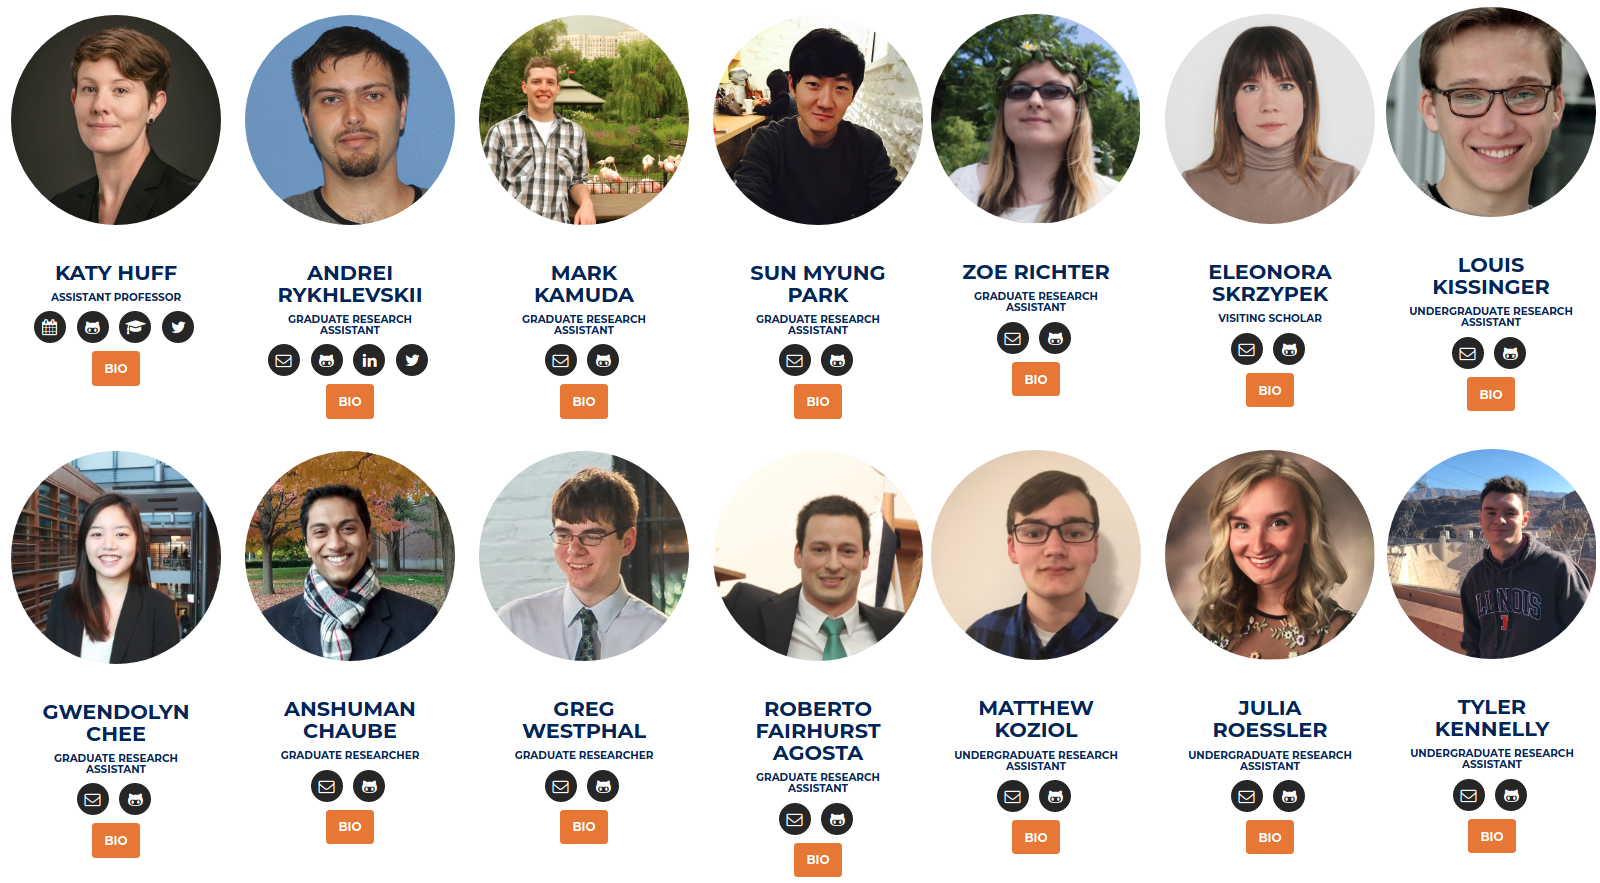
\includegraphics[height=0.63\textwidth]{./images/arfc1.png}
                \caption{Current Advanced Reactors and Fuel Cycles Group researchers.}
               \end{figure}            
\end{frame}

\begin{frame}
  \frametitle{Advanced Reactors and Fuel Cycles group (PI: Kathryn Huff)}
               \begin{figure}[t]
                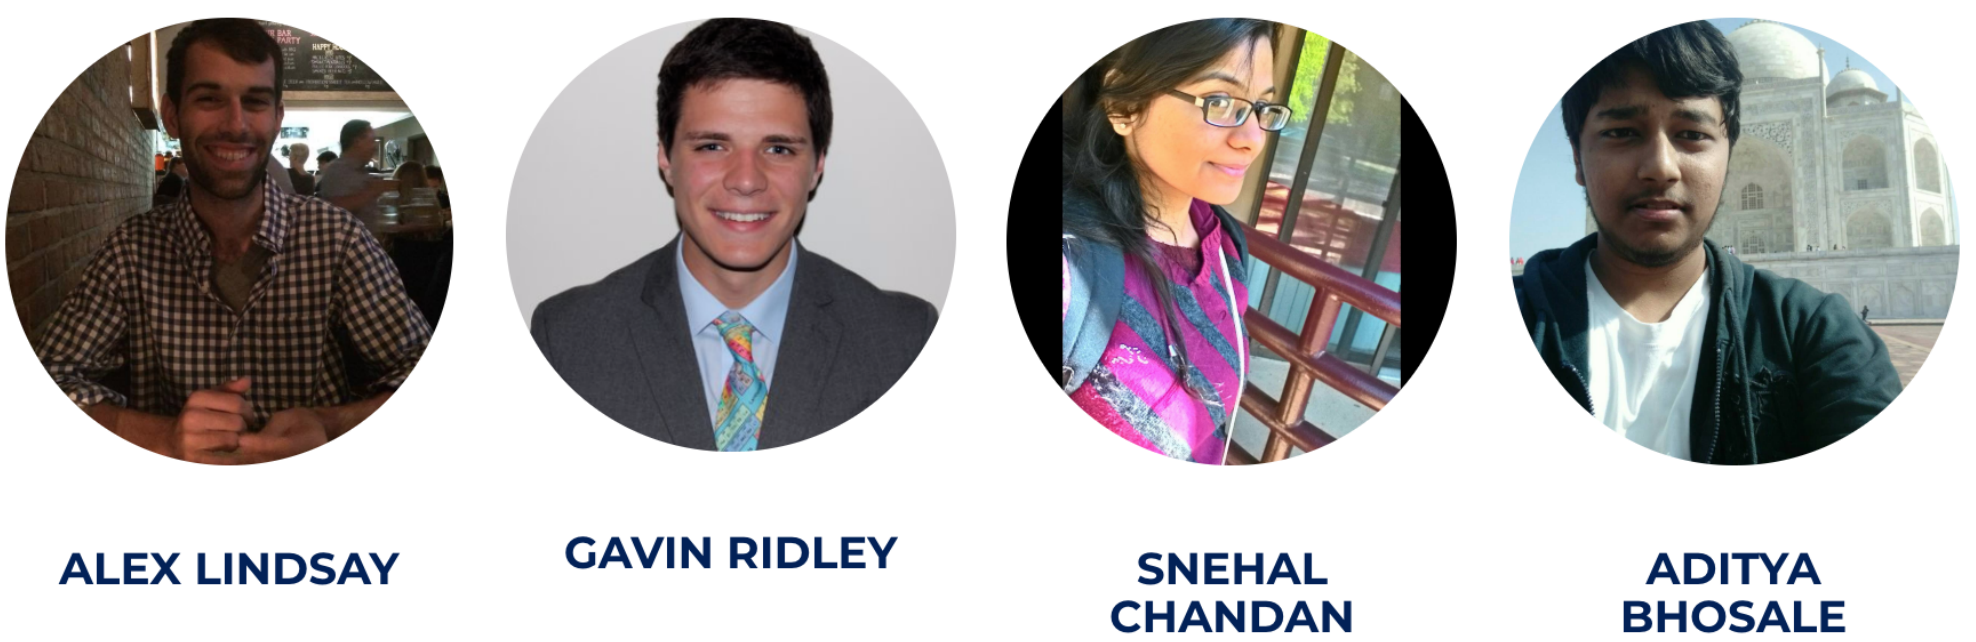
\includegraphics[height=0.33\textwidth]{./images/arfc_past.png}
                \caption{Past ARFC Group members who contributed to this work.}
               \end{figure}            
\end{frame}


\begin{frame}
  \frametitle{Insights at Disparate Scales}
               \begin{figure}[t]
                \vspace*{-0.1in}
			\hspace*{-0.35in}
                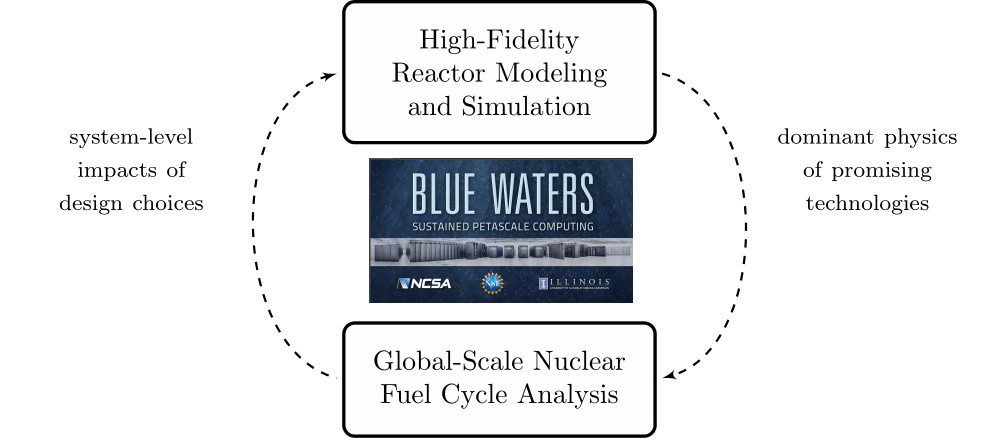
\includegraphics[height=0.5\textwidth]{./images/synergy.png}
               \end{figure}            
\end{frame}

\subsection{Molten salt reactors}
\begin{frame}
  \frametitle{Molten Salt Reactor Types}
                  \vspace*{-0.1in}
              \begin{block}{Stationary Fuel}
               \begin{enumerate}
                \item Graphite block with TRISO fuel, clean salt works as coolant (e.g. TMSR-SF1, FHR-DR)
                \item Plate Fuel: hexagonal fuel assembly is similar in shape to a typical sodium-cooled reactor
                        % Not sure what FIRM is.
                %\item Fuel Inside Radial Moderator (FIRM)
                        % While it doesn't leave the reactor, doesn't 
                        % the fuel in the moltex reactor move up and down?
                        % If the fluid is free to naturally circulate inside 
                        % the rod, it likely happens on 
                        % timescales that I do not think we can ignore from a 
                        % kinetics perspective. 
                %\item Liquid fuel salt inside fuel rods cooled by clean salt (e.g. Moltex Stable Salt Reactor)
               \end{enumerate}
               \end{block}
               
               \begin{block}{Mobile Fuel}
               \begin{enumerate}
                \item Mobile solid fuel elements (e.g. pebbles) cooled by clean salt (e.g. PB-FHR)
                \item Non-circulating liquid fuel salt (e.g. TerraPower MCFR) 
                \item \textbf{Circulating fuel salt} which also works as coolant (e.g. \gls{MSRE}, \gls{MSBR}, TAP MSR)
               \end{enumerate}
               \end{block}
\end{frame}

\begin{frame}
  \frametitle{Stationary and Mobile Solid fuel}
        \vspace*{-0.1in}
               \begin{figure}[t]
			\hspace*{-0.35in}
                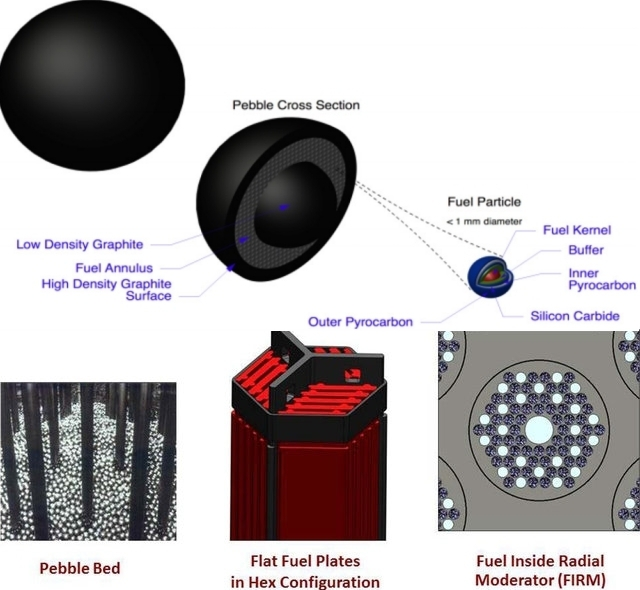
\includegraphics[height=0.63\textwidth]{./images/solid_fuel.jpg}
                \caption{TRISO fuel particle (top) and FHR fuel designs (bottom). Source \cite{forsberg_basis_2016-1}.}
             \end{figure}   
  
\end{frame}

\begin{frame}
  \frametitle{Mobile, Non-Circulating, Liquid Fuel}
               \begin{figure}[t]
                \vspace*{-0.1in}
			\hspace*{-0.35in}
                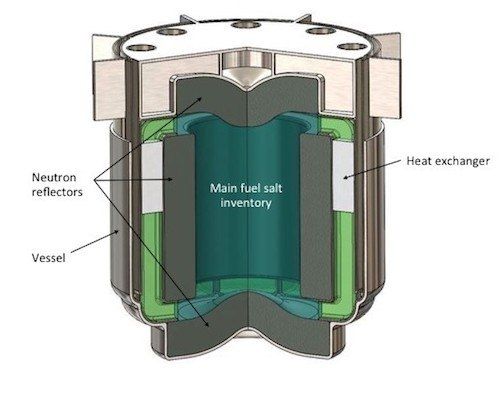
\includegraphics[height=0.6\textwidth]{./images/mcfr-crossection.jpg}
                \caption{The TerraPower MCFR is an example of reactor design with \textbf{liquid, mobile, non-circulating} chloride salt fuel. Source \cite{doene_southern_2018}.}
             \end{figure}   
  
\end{frame}

\begin{frame}
  \frametitle{Mobile, Circulating, Liquid Fuel}
               \begin{figure}[t]
                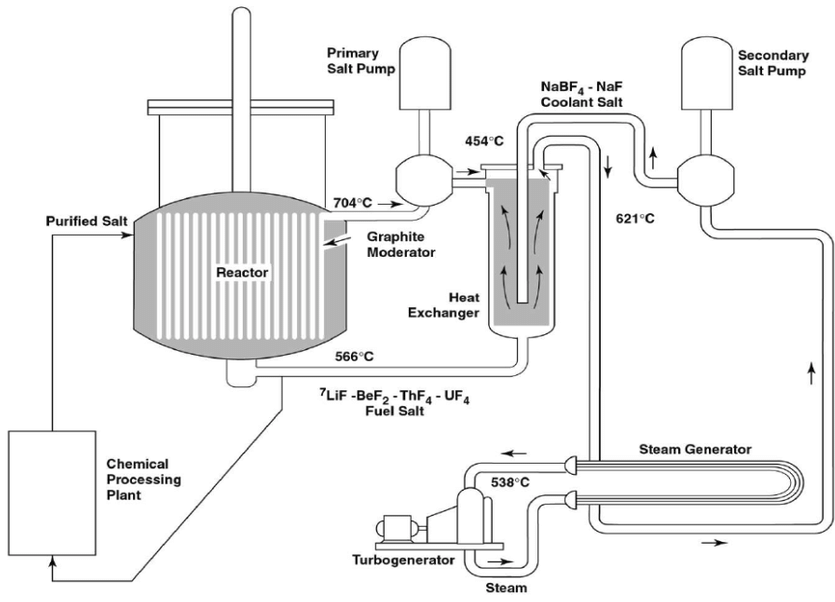
\includegraphics[height=0.58\textwidth]{./images/msbr_scheme.png}
                \caption{The \gls{MSBR} is an example of reactor design with \textbf{liquid, mobile, circulating} fluoride salt fuel \cite{rosenthal_molten-salt_1970}.}
             \end{figure}   
  
\end{frame}

\subsection{Motivation}
\begin{frame}
  \frametitle{Why Molten Salt Reactors with circulating fuel?}
              \begin{block}{Main advantages of liquid-fueled \glspl{MSR} \cite{elsheikh_safety_2013}}
               \begin{enumerate}
                \item High coolant temperature (600-750$^{\circ}$C)
                \item Fuel diversity ($^{235}$U, $^{233}$U, Thorium, U/Pu)
                \item Increased inherent safety
                \item High fuel utilization $\Rightarrow$ less nuclear waste generated
                \item Online reprocessing and refueling
                \item Thermal/epithermal (\gls{MSBR}) or fast spectrum (\gls{MSFR})
                \item Can produce more fissile material than it consumes (breeder)
                \item Nuclear Spent Fuel Transmuter (e.g. REBUS-3700 \cite{mourogov_potentialities_2006-1}, MOSART \cite{ignatiev_molten_2014}) 
               \end{enumerate}
               \end{block}

\end{frame}

\begin{frame}
  \frametitle{Challenges in \gls{MSR} Simulation}
                  \vspace*{-0.05in}
               \begin{enumerate}
                \item Contemporary burnup codes cannot treat fuel movement
                \item Neutron precursor location is hard to estimate
                \item Operational and safety parameters change during reactor operation
                \item Power generation strongly depends on fuel temperature and vica versa
               \end{enumerate}

           \begin{figure}[t]
                \vspace*{-0.05in}
			\hspace*{-0.2in}
                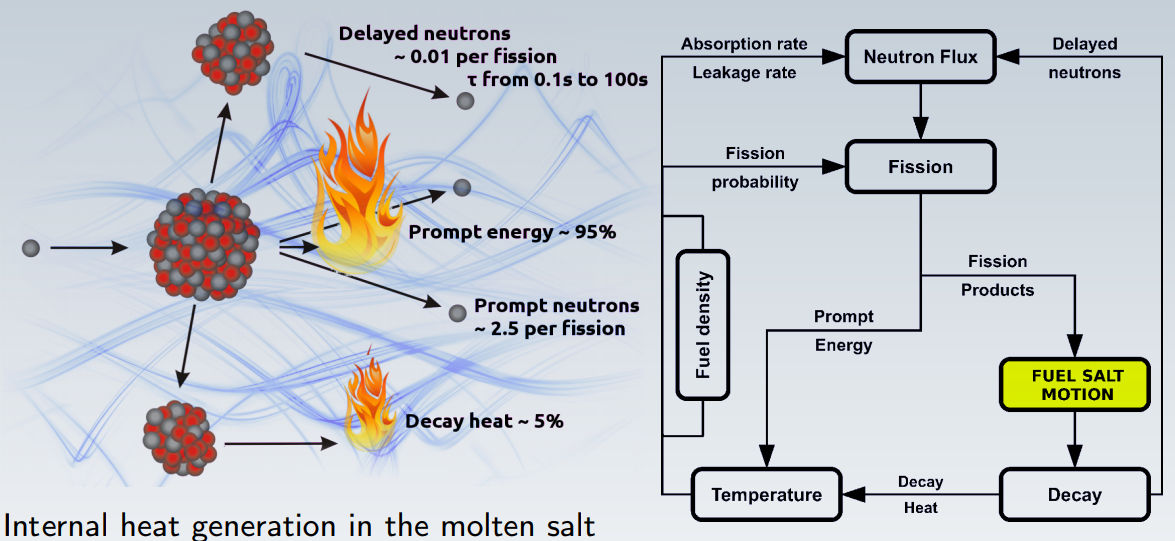
\includegraphics[height=0.47\textwidth]{./images/coupled_physics.png}
		\vspace*{-0.05in}
		\caption{Challenges in simulating \glspl{MSR} (Image courtesy of Manuele Aufiero,2012).}
     	 \end{figure}               
\end{frame}

\begin{frame}
  \frametitle{Research objectives}
                  \vspace*{-0.1in}

              \begin{block}{Multiphysics simulation of \gls{MSR} (Moltres/MOOSE)\cite{lindsay_introduction_2018}}
               \begin{enumerate}
                \item Demonstrate steady-state and transient coupling of neutron fluxes, precursor drift, and thermal-hydraulics
                \item Implement advective movement of delayed neutron precursors
                \item Demonstrate capabilities with 2D axisymmetric and 3D mesh
                \item Simple transients: change of flow and moderator movement
               \end{enumerate}
               \end{block}


              
\end{frame}

\section{Methodology}
\subsection{Fuel salt reprocessing system}

\begin{frame}
  \frametitle{Fuel salt reprocessing system overview: gas separation}
  Gaseous fission products (e.g., Xe, Kr) must be removed from the fuel salt 
  to avoid reactor
poisoning. 
  
      \begin{columns}
      	\column[t]{4.7cm}
    \begin{block}{Noble gas removal}
      \begin{enumerate}
      	\item bubble generator injects He bubbles in the salt stream
      	\item noble gas migrate to the He bubbles 
      	\item gas separator discharges the poison-rich bubbles
      \end{enumerate}
    \end{block}    	
      	
     	\column[t]{8cm}
  \begin{figure}[t]
	  \centering
	  		\vspace{-8mm}
		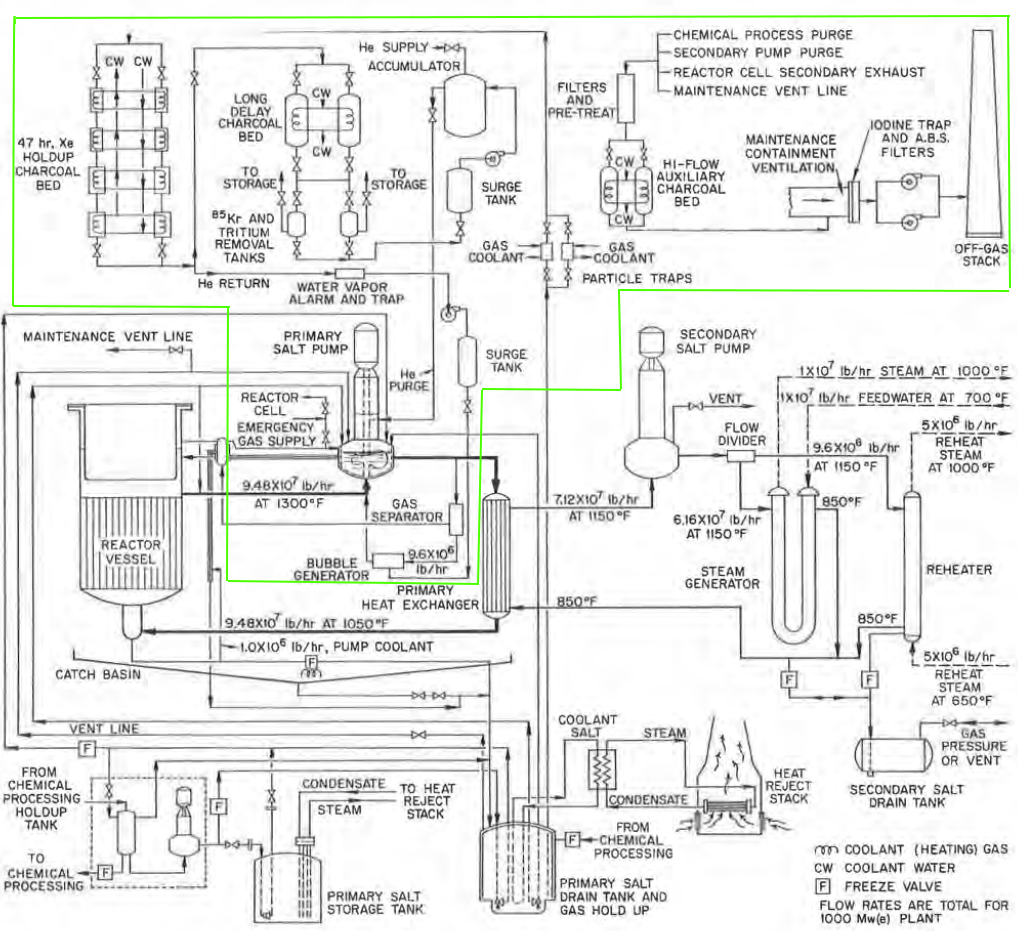
\includegraphics[width=\textwidth]{../figures/gas_separation.pdf}
	\caption{Schematic flow diagram of the \gls{MSBR} gas separation system 
	(figure reproduced from Robertson \emph{et al.}  
	\cite{robertson_conceptual_1971}).} 
    \end{figure}

	\end{columns}
\end{frame}

\begin{frame}
  \frametitle{Mathematical model for gas separation efficiency}
  		\vspace{-1mm}
Xenon removal efficiency ($\epsilon_{Xe}$) in a gas separation system is 
\cite{peebles_removal_1968}:
\begin{align}
& \qquad\qquad \epsilon_{Xe} = \frac{1-e^{-\beta}}{1+\alpha} \nonumber \\
\alpha &= \frac{RTQ_{L}}{HQ_{G}} \nonumber \\
\beta &= \frac{K_L a A_C L (1+\alpha)}{Q_{L}} \nonumber \\
Q_{L}&= \mbox{volumetric salt flow rate} \nonumber \\
Q_{G}&= \mbox{volumetric helium flow rate} \nonumber \\
H &= \mbox{Henry's law constant} \nonumber \\
a &= \mbox{gas-liquid interfacial area} \nonumber \\
K_L &= \mbox{liquid phase mass transfer coefficient.} \nonumber
\end{align}
		\vspace{-5mm}
  \begin{figure}[t]
	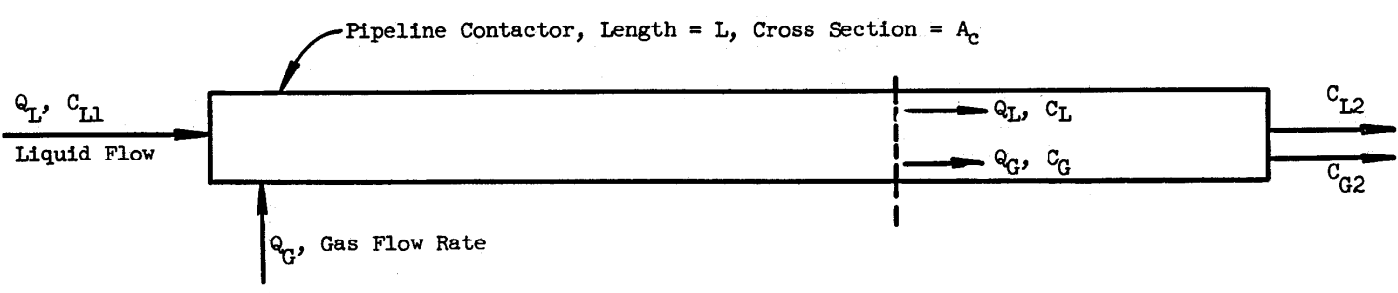
\includegraphics[width=0.66\textwidth]{./images/pipeline_contactor.png}
	\vspace{-2mm}
	\caption{Flow diagram for gas separator (figure reproduced from Peebles 
		\emph{et al.} \cite{peebles_removal_1968}).}
\end{figure}

\end{frame}


\begin{frame}
\frametitle{Fuel processing system overview: rare earths and Pa removal}
	\begin{figure}[htp!] % replace 't' with 'b' to 
		\centering
			\includegraphics[width=0.57\textwidth]{../figures/flowsheet.pdf}
			\vspace{-2mm}
		\caption{Liquid metal (Bi) extraction system for the \gls{MSBR} 
		(reproduced from Sorensen \cite{sorensen_one-fluid_2006}).} 
	\end{figure}
	
\end{frame}


\begin{frame}
\frametitle{Fuel processing system overview: TAP concept}
	\vspace{-2mm}
\begin{figure}[htp!] % replace 't' with 'b' to 
	\centering
	\includegraphics[width=0.75\textwidth]{../figures/tap_primary_loop.png}
	\caption{Simplified \gls{TAP} primary loop design including off-gas system 
		(blue), nickel filter (orange) and liquid metal extraction system 
		(green) \cite{transatomic_power_transatomic_2019}.}
\end{figure}

\end{frame}


\begin{frame}
\frametitle{SaltProc demonstration for TAP concept input data}
	  \begin{textblock*}{12.5cm}(0.5cm,1.5cm) % {block width} (coords)
%%%%%%%%%%%%%%%%%%%%%%%%%%%%%%%%%%%%%%%%
\begin{table}[htbp!]
	\fontsize{6}{9}\selectfont
	\centering
	\caption{The effective cycle times for fission products removal  from the 
		\gls{TAP} reactor \cite{betzler_implementation_2017}.}
	\begin{tabular}{p{0.14\textwidth} p{0.3\textwidth} p{0.11\textwidth} 
			p{0.11\textwidth}}
		\hline 
		\textbf{Processing group} & \qquad\qquad\qquad \textbf{Nuclides} & 
		\textbf{Removal Rate (s$^{-1}$)} & \textbf{Cycle time (at full power)} 
		\\ \hline 
		\multicolumn{3}{c}{\textit{Elements removed in \gls{MSBR} concept and 
				adopted for the \gls{TAP}} \cite{robertson_conceptual_1971}} \\
		Noble gases & Xe, Kr								  & 5.00E-2 & 20 
		sec \\
		Noble metals & Se, Nb, Mo, Tc, Ru, Rh, Pd, Ag, Sb, Te & 5.00E-2 & 20 
		sec \\
		Seminoble metals & Zr, Cd, In, Sn	  				  & 5.79E-8 & 200 
		days\\
		Volatile fluorides & Br, I 							  & 1.93E-7 & 60 
		days\\
		Rare earths & Y, La, Ce, Pr, Nd, Pm, Sm, Gd           & 2.31E-7 & 50 
		days\\
		\qquad & Eu & 2.32E-8 & 500 days \\
		Discard & Rb, Sr, Cs, Ba & 3.37E-9 & 3435 days \\
		\hline
		\multicolumn{3}{c}{\textit{Additional elements removed} 
			\cite{betzler_implementation_2017, 
			transatomic_power_corporation_neutronics_2016}} \\
		Noble gases & H								  	& 5.00E-2 & 20 
		sec    \\
		Noble metals & Ti, V, Cr, Cu						& 3.37E-9 & 3435 
		days \\
		Seminoble metals & Mn, Fe, Co, Ni, Zn, Ga, Ge, As   & 3.37E-9 & 3435 
		days \\
		Rare earths & Sc									& 3.37E-9 & 3435 
		days \\
		Discard & Ca										& 3.37E-9 & 3435 
		days \\
		\hline
	\end{tabular}
	\label{tab:reprocessing_list}
\end{table}
	\begin{itemize}
		\item Noble gas removal efficiency: variable, described using 
		mathematical 
		correlation
		\item Other FP removal efficiency: fixed, non-ideal, based on 
		Table~\ref{tab:reprocessing_list}
	\end{itemize}
	\end{textblock*}
\end{frame}


\subsection{Proposed tool design}


\begin{frame}
\frametitle{SaltProc class architecture}
	\begin{itemize}
		\item \textit{Simulation} class
			\begin{itemize}
				\item Manages simulation process
				\item Stores data into the HDF5 database
				\item Tracks time
			\end{itemize}
		\item \textit{Depcode} class
			\begin{itemize}
				\item Contains attributes and methods for reading user's input
				\item Creates input files for depletion code
				\item Parses depletion code output 
			\end{itemize}
		\item \textit{Process} class
			\begin{itemize}
				\item Represents fuel processing system component
				\item Contains attributes of the component ($\epsilon_e$, throughput rate, capacity)
				\item Tracks waste stream
			\end{itemize}
		\item \textit{MaterialFlow} class
			\begin{itemize}
				\item Instances of that class represents the material flowing between processes
			\end{itemize}
	\end{itemize}
		\vspace{3mm}
	\begin{figure}[ht!] % replace 't' with 'b' to 
		\centering
		\includegraphics[width=0.6\textwidth]{../figures/materialflow.pdf}
		\vspace{-0.1in}
		\caption{Schematic for passing material data between fuel processing 
		system components.}
	\end{figure}

\end{frame}


\begin{frame}
\frametitle{SaltProc flowchart}
\vspace{-2mm}
\begin{figure}[ht!] % replace 't' with 'b' to \centering
	\centering
	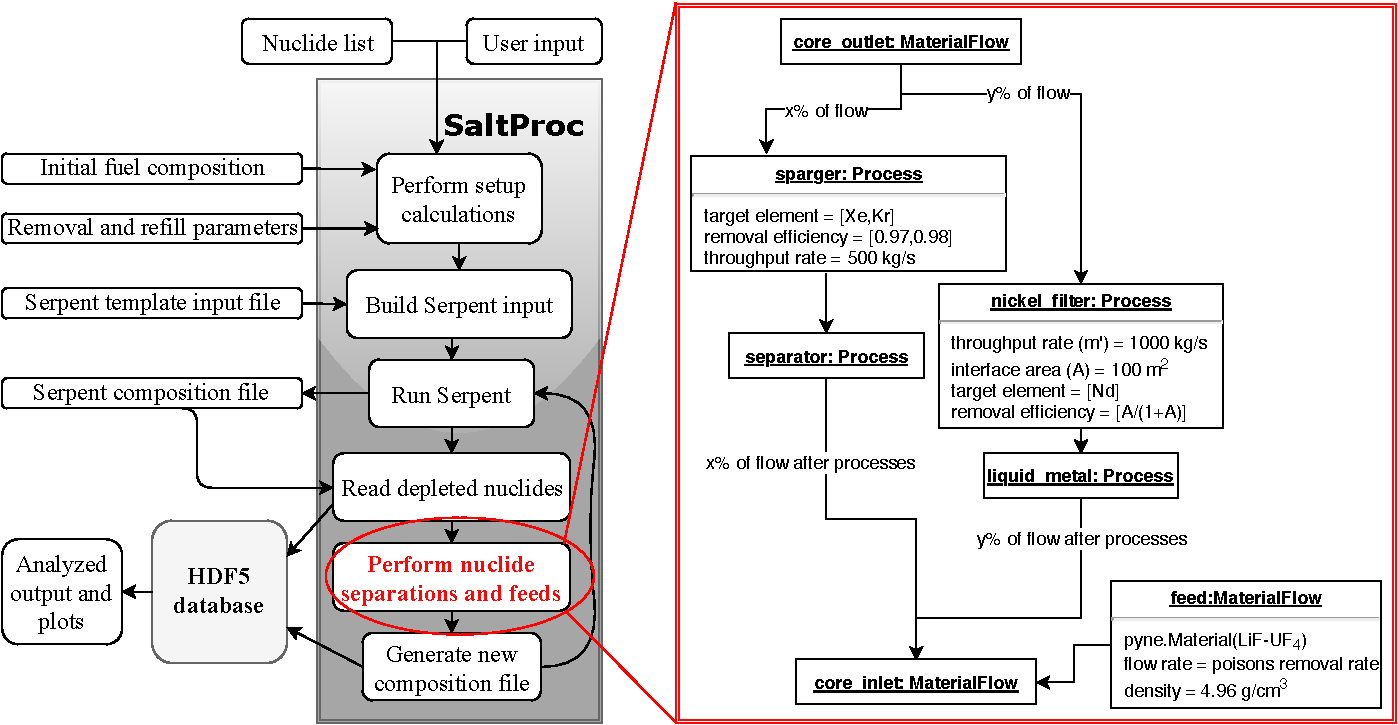
\includegraphics[width=1.05\textwidth]{./images/saltproc_flowchart.pdf}
	\caption{Tentative generic flowchart for SaltProc v1.0 python package.}
\end{figure}

\end{frame}
\section{Preliminary results}
\subsection{Proposed work plan}

\begin{frame}
  \frametitle{Progress chart}       
  	  \begin{textblock*}{12.5cm}(0.1cm,2.2cm) % {block width} (coords)
 \begin{figure}[ht!] % replace 't' with 'b' to force it to 
	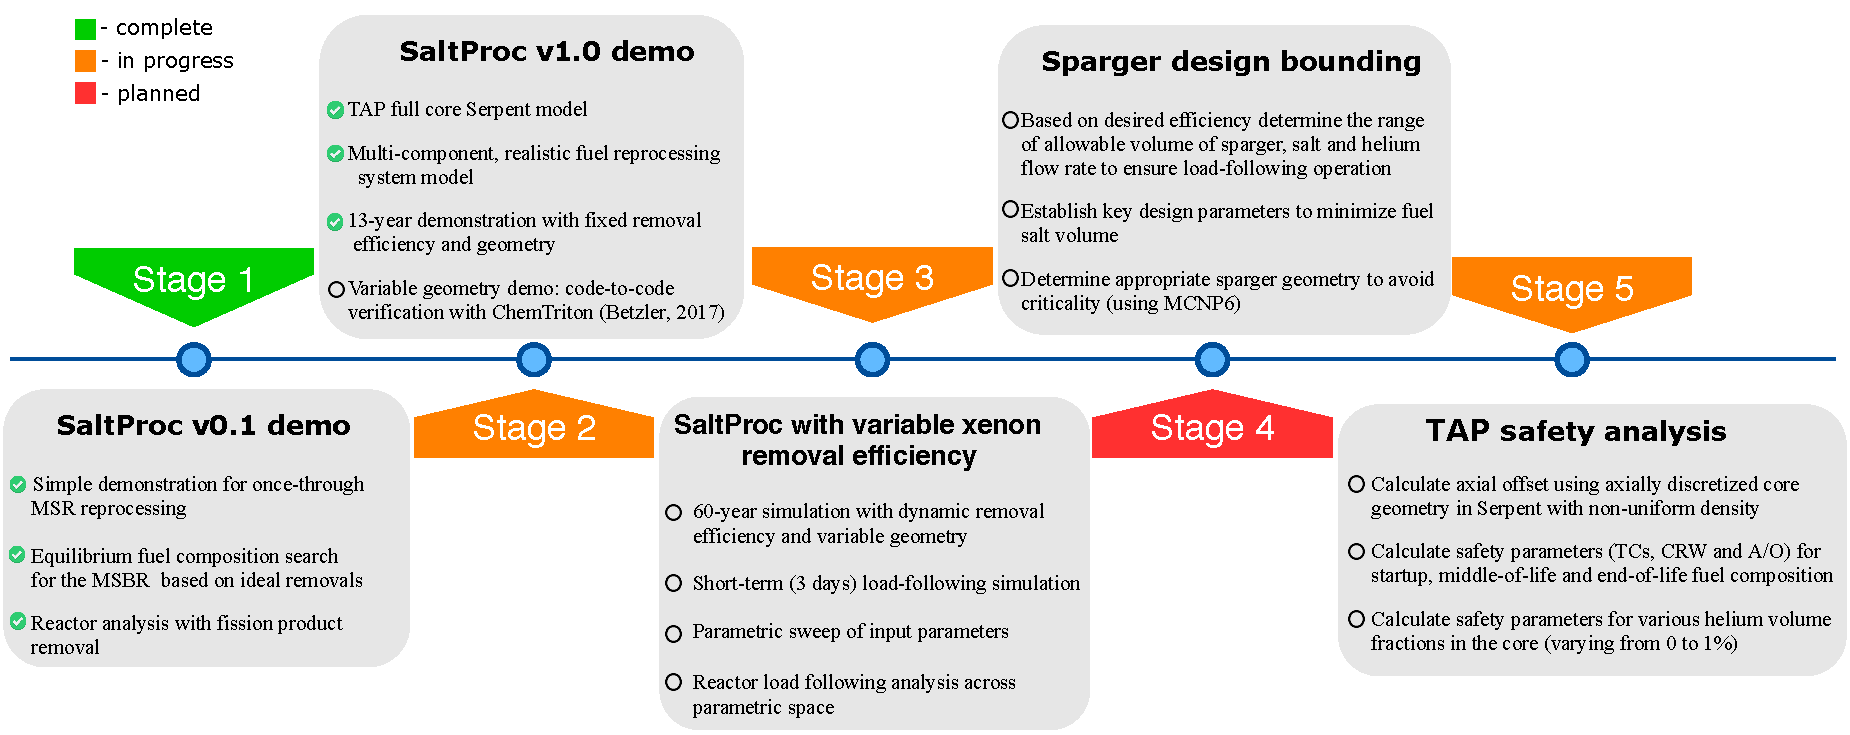
\includegraphics[width=\textwidth]{./images/progress_chart.pdf} 
	\caption{Workflow for the simulations proposed in this work.}
\end{figure}
		\end{textblock*}
\end{frame}


\subsection{Stage 1: Basic on-line reprocessing demonstration}

\begin{frame}
\frametitle{MSBR online reprocessing analysis}

\begin{columns}
	\column[t]{4.3cm}
	\begin{block}{SaltProc v0.1 demo for simple once-through \gls{MSR} 
	reprocessing}
		\fontsize{7}{9}\selectfont
		\begin{itemize}
			\item Full-core model of the \gls{MSBR} for 60 years of operation
			\item FP removal from the salt with fixed, ideal extraction 
			efficiencies 
			\item $^{233}$Pa ideal removal and feed of an equal mass of 
			$^{233}$U into the core
			\item Fresh fertile material feed to maintain the salt inventory
			\item Fine time resolution (3-day depletion steps)
		\end{itemize}
	\end{block}    	
	
	\column[t]{8cm}
		\begin{figure}[ht!] 
		\centering
			\includegraphics[width=\textwidth]{../figures/keff_msbr.png}
			\caption{Effective multiplication factor dynamics for the 
			full-core \gls{MSBR} model (reproduced from  
			Rykhlevskii \emph{et al.} \cite{rykhlevskii_modeling_2019}).}
		\end{figure}
	
\end{columns}
\end{frame}


\begin{frame}
\frametitle{Effect of fission products removal}       

\begin{figure}[t] % replace 't' with 'b' to force it to 
	\centering
	\includegraphics[width=0.8\textwidth]{../figures/keff_rem_cases.png} 
	\caption{Calculated effective multiplication factor for the full-core 
		\gls{MSBR} model with removal of various fission product groups over 
		10 	years of operation (reproduced from Rykhlevskii \emph{et al.} 
		\cite{rykhlevskii_modeling_2019}).}
\end{figure}

\end{frame}


\subsection{Stage 2: Tool demonstration and validation for \gls{TAP}}

\begin{frame}
\frametitle{\gls{TAP} concept high-fidelity Serpent model}
	  \begin{textblock*}{12.25cm}(0.25cm,1.8cm) % {block width} (coords)
\begin{figure}[htp!] % replace 't' with 'b' to 
	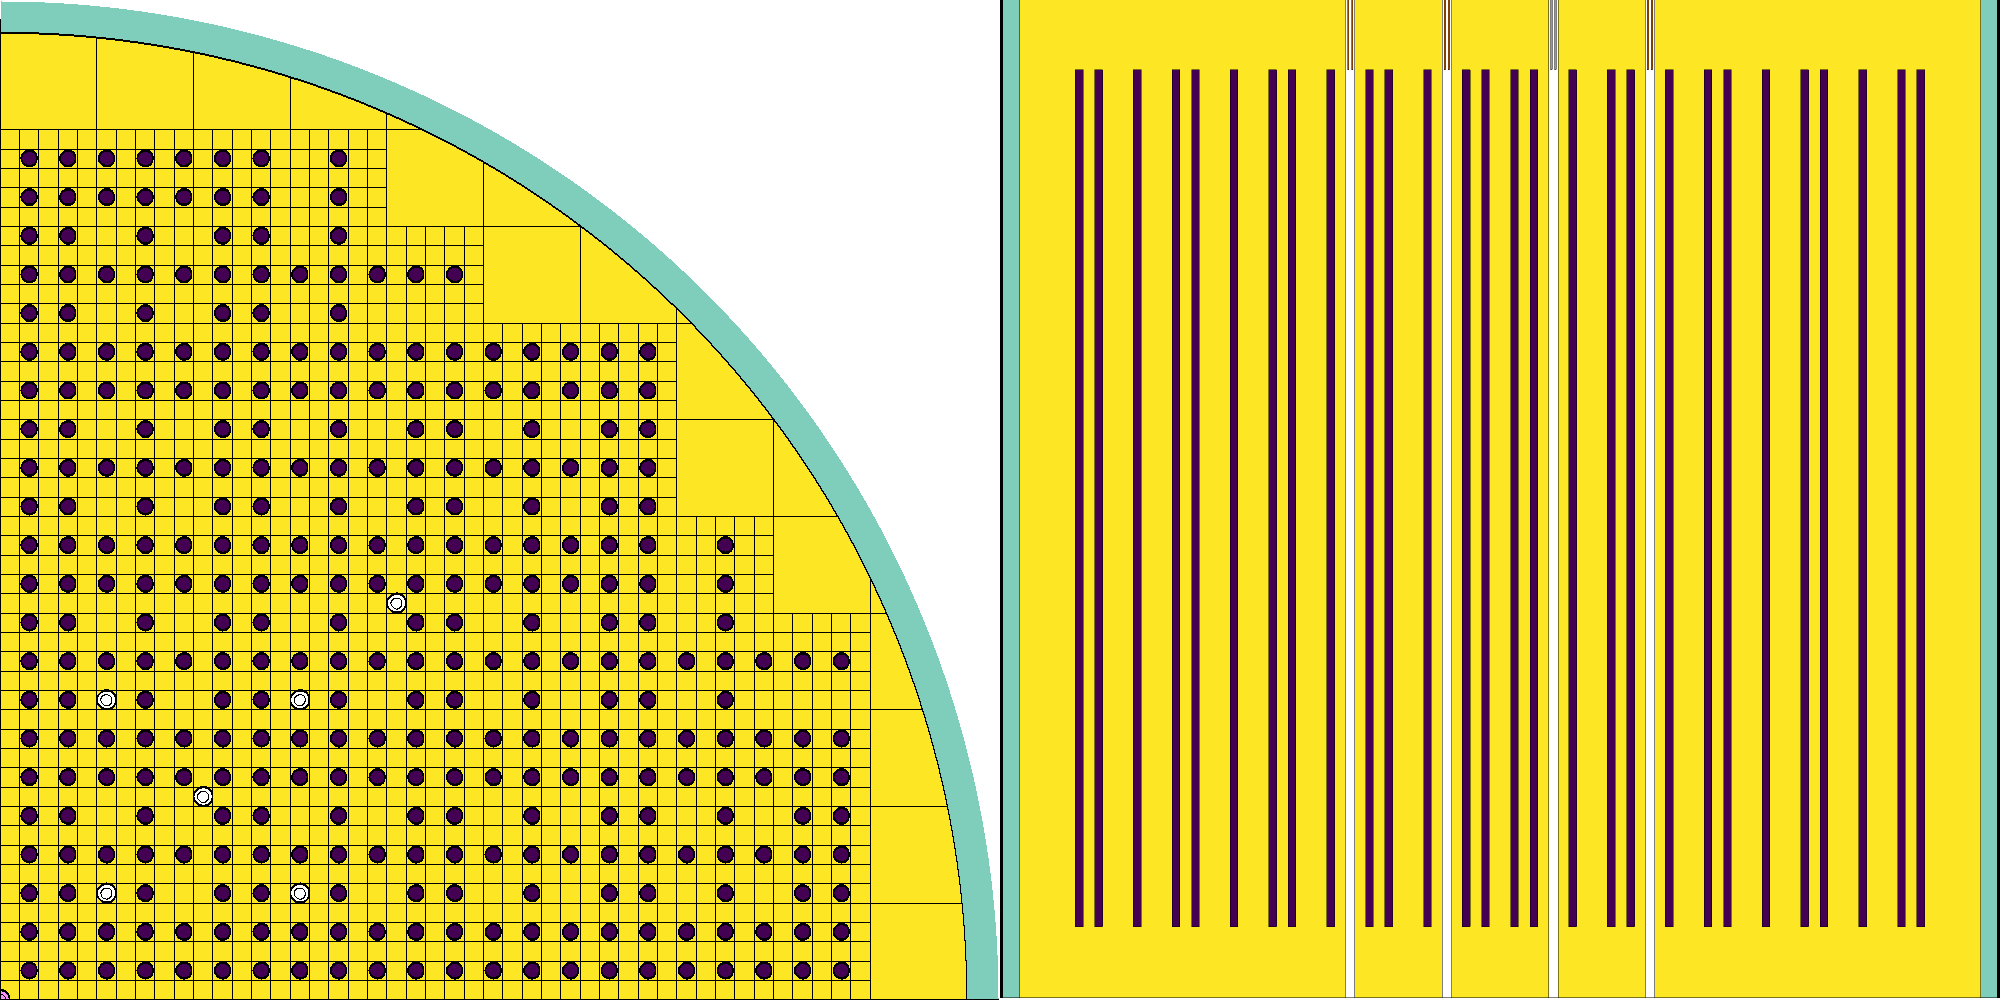
\includegraphics[width=\textwidth]{./images/tap_model.png}
	\caption{An $XY$ (left) and $XZ$ (right) section of the \gls{TAP} model. 
	The violet color represents
zirconium hydride, and the yellow represents 
	fuel salt 
	(reproduced from Rykhlevskii \& Huff \cite{rykhlevskii_milestone_2019}).}
\end{figure}
	  \end{textblock*}
\end{frame}


\begin{frame}
\frametitle{Multi-component fuel reprocessing system model in SaltProc}       

\begin{columns}
		\column[t]{6cm}
		\begin{itemize}
			\item Fixed, non-ideal ($<100\%$) removal efficiencies
			\item Sparger and separator located in-line
			\item Static geometry with constant moderator-to-fuel ratio
			\item 5\% and 19.79\% low-enriched uranium feed
		\end{itemize}

	\column[t]{6.5cm}
	\begin{figure}[htp!] % replace 't' with 'b' to 
	\centering
			\vspace{-7mm}
		\begin{overprint}
	\onslide<1>\includegraphics[height=0.8\textheight]{../figures/demo_reprocessing_scheme.png}
	\onslide<2>\includegraphics[height=0.8\textheight]{../figures/demo_reprocessing_scheme_2.png}
		\end{overprint}
	\caption{\gls{TAP} reprocessing scheme flowchart used for demonstration of 
		SaltProc \cite{rykhlevskii_milestone_2019}.}
	\end{figure}
\end{columns}
\end{frame}


\begin{frame}
\frametitle{Depletion simulation results for TAP with various feeds}       
\begin{textblock*}{12.6cm}(0.1cm,2.2cm) % {block width} (coords)
	\begin{figure}[htp!] % replace 't' with 'b' to 
		\begin{minipage}[b]{0.48\textwidth}
			\includegraphics[width=\linewidth]{../figures/keff_3.png}
		\end{minipage}
			\hspace{-2mm}
		\begin{minipage}[b]{0.48\textwidth}
			\includegraphics[width=\linewidth]{../figures/keff_zoomed_2.png}
		\end{minipage}
		\caption{Effective multiplication factor dynamics for full-core
		\gls{TAP} model for different fueling scenarios over a 13-year reactor 
		operation (left) and for the time interval from 367 to 471 days after 
		startup (right). Confidence interval $\pm\sigma=28pcm$ is shaded.}
	\end{figure}
\end{textblock*}
\end{frame}


\begin{frame}
\frametitle{Fuel salt composition evolution during the TAP operation}
\begin{textblock*}{12.25cm}(0.25cm,1.8cm) % {block width} (coords)
	\begin{figure}[htp!] % replace 't' with 'b' to 
		\centering
				\vspace{-3mm}
		\includegraphics[width=0.72\textwidth]{../figures/u_pu_mass.png}
		\caption{Mass of major nuclides during 13 years of reactor operation 
		with 19.79\% \gls{LEU} feed.}
	\end{figure}
\end{textblock*}
\end{frame}


\subsection{Stage 5: Safety parameters evolution}

\begin{frame}
\frametitle{Safety parameters calculations at start-up}       

\begin{columns}
	\column[t]{6cm}
	\begin{itemize}
		\item \gls{TAP} reactor operation range is 773-973K
		\item Temperature coefficient of reactivity calculated separately for 
		fuel and moderator in range 800-1000K
		\item Temperature coefficients are negative at start-up but are 
		expected to be more negative during operation
		\item A configuration of 25 control rods has a reactivity worth of 
		$1110\pm9.7$pcm (1.1\%) at startup
		\item Serpent template to calculate temperature coefficients and  
		control rod worth by single run was developed
	\end{itemize}
	
	\column[t]{6.5cm}
	\begin{figure}[bth!] % replace 't' with 'b' to 
	\includegraphics[width=\textwidth]{../figures/axial_offset.png}
	\caption{\gls{TAP} model divided to multiple axial layers with different 
	densities of the salt to calculate axial power offset.}
	\end{figure}
\end{columns}
\end{frame}


\section{Future work}
\begin{frame}
\frametitle{Additional simulation and analysis}       
\begin{textblock*}{12.5cm}(0.1cm,2.2cm) % {block width} (coords)
	\begin{figure}[ht!] % replace 't' with 'b' to force it to 
		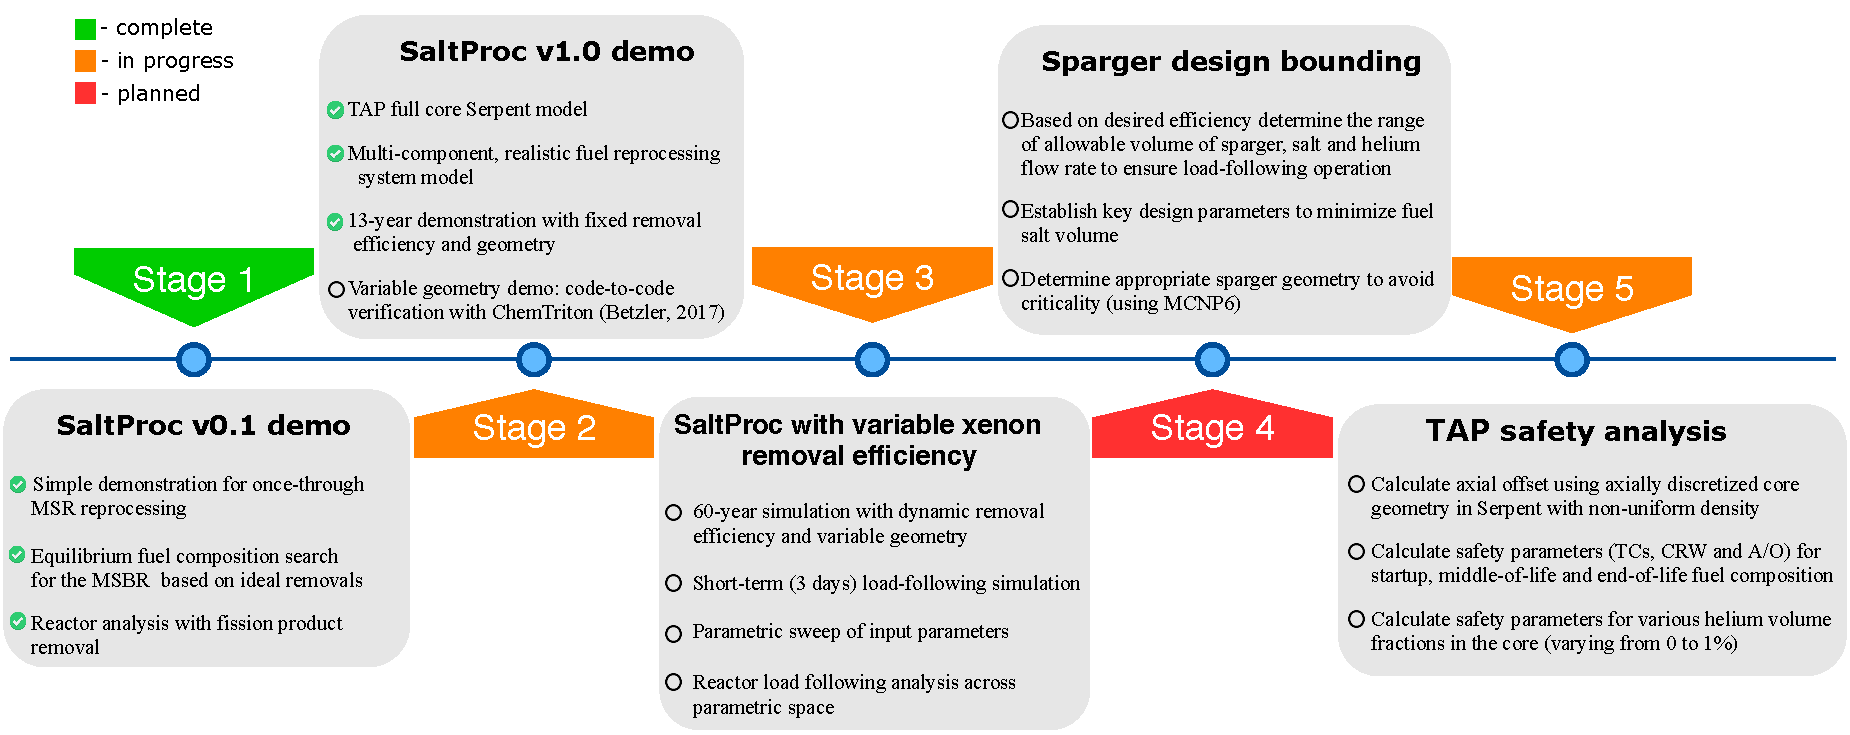
\includegraphics[width=\textwidth]{./images/progress_chart.pdf} 
	\end{figure}
\end{textblock*}
\end{frame}


\begin{frame}
\frametitle{SaltProc demonstration for realistic on-line reprocessing system}
	\begin{block}{Finishing Stage 2}
		\begin{enumerate}
			\item Implement variable core geometry capability in SaltProc
			\item Demonstrate a key feature of
the \gls{TAP} reactor - 
			adjusting the moderator rod configuration - which is necessary 
			achieve 60-years lifetime.
			\item Perform 40-year depletion simulation using SaltProc 
			and compare obtained results with Betzler \emph{et al.} 
			\cite{betzler_assessment_2017}
		\end{enumerate}
	\end{block}
	
	\begin{block}{Stage 3: SaltProc demonstration with variable Xe removal 
	efficiency}
		\begin{enumerate}
			\item Incorporate extraction efficiencies as a function of many 
			physical system design
parameters (e.g., void fraction in the 
			salt, helium bubble size)
			\item Perform life-time long depletion simulation with dynamic 
			removal efficiency
			\item Perform short-term (3 days) depletion with the core power 
			changing in the [0, 100\%] range with a ramp rate 10\%/min
			\item Conduct parametric sweep of input parameters in the xenon 
			extraction equation to determine the range of key parameters when 
			load-following is possible
		\end{enumerate}
	\end{block}
\end{frame}


\begin{frame}
\frametitle{Gas removal system bounding and safety analysis for the TAP}
\begin{block}{Stage 3: Prototype design for the Xe removal system}
	\begin{enumerate}
		\item Determine bounds for key design parameters (sparger volume, 
		geometry, salt and helium flow rates) by analyzing parametric sweep
		\item Calculate key design parameters to minimize fuel salt inventory 
		in the system
		\item Perform nuclear criticality safety analysis using MCNP6 
		\cite{werner_mcnp6._2018} to
confirm that the selected 
		sparger design is safe
	\end{enumerate}
\end{block}

\begin{block}{Stage 5: \gls{TAP} Safety and Operational parameters analysis}
	\begin{enumerate}
		\item Finish a axially discretized core
geometry in Serpent with 
		non-uniform axial density distribution to estimate the axial power
		offset
		\item Calculate safety parameters (temperature coefficients, control 
		rod worth, axial power offset) at the \gls{BOL}, the middle-of-life, 
		and the \gls{EOL}
		\item Repeat for short-term depletion to capture the parameters 
		dynamics for load-following operation
	\end{enumerate}
\end{block}
\end{frame}


\begin{frame}
\frametitle{Conclusion}
	\begin{textblock*}{12cm}(0.4cm,2cm) % {block width} (coords)
	\begin{itemize}
		\item Motivation for the developing fuel processing simulation tool 
		for liquid-fueled nuclear reactors have been outlined
		\begin{itemize}
			\item Fuel salt processing systems modeling in \glspl{MSR} have 
			historically been conceptual rather than concrete
			\item This work will more realistically model salt processing 
			system with a focus
on the gas removal system of the prospective 
			\gls{TAP} \gls{MSR}
		\end{itemize} 
		\item Preliminary results obtained using SaltProc include:
			\begin{itemize}
				\item Simple demonstration for \gls{MSBR} with ideal/fixed 
				fission products removal efficiency
				\item Multi-component fuel reprocessing system modeling 
				for \gls{TAP} with non-ideal/constant efficiency
				\item Determining the effect of fission product removal on the 
				core neutronics
			\end{itemize}
		
		\item Future work
			\begin{itemize}
				\item Add variable geometry and dynamic removal efficiency 
				capability to realistically model the \gls{TAP} system
				\item Demonstrate and validate those capabilities for 
				lifetime-long depletion simulations
				\item Simulate the \gls{TAP} reactor behavior in short-term 
				transients to determine the
feasibility of load following
				\item Determine feasible design parameters of the sparger, 
				critical component of the
TAP gas removal system
				\item Analyze dynamics of the safety parameters for long-term 
				and short-term cases
			\end{itemize}
	\end{itemize}
\end{textblock*}
\end{frame}

%%--------------------------------%%
%%--------------------------------%%
\begin{frame}[allowframebreaks]
  \frametitle{References}
  \bibliographystyle{unsrt}
  {\footnotesize \bibliography{../thesisrefs.bib} }

\end{frame}

%%--------------------------------%%
%%---BACKUP SLIDES----------------%%
\begin{frame}
\frametitle{SaltProc architecture}
\vspace{-2mm}
\begin{figure}[ht!] % replace 't' with 'b' to \centering
	\includegraphics[width=0.84\textwidth]{../figures/saltproc_class_diagram.png}
	\caption{SaltProc v1.0 python package class diagram in UML notation 
		with examples of object instances.}
\end{figure}

\end{frame}	



\end{document}



